%% Latex Preamble

 \documentclass[11pt,dvipsnames]{article} % can use article for american style of headings (scrartcl for European)
%\usepackage[margin=2.5cm]{geometry} % sets the borders to 3cm each

%My modification
\RequirePackage[
paperwidth		=8.5in,
paperheight		=11in,
top				=0.5in, 
bottom			=0.75in, 
left			=0.75in, 
right			=0.75in
]{geometry}


\usepackage[english]{babel}     %defines language for spacing
\usepackage[utf8]{inputenc}   % allows entering special characters
\usepackage[T1]{fontenc}        % sets font to T1 and allows umlaute
\usepackage{lmodern}            % improves font display in PDFs
\usepackage{microtype}          % improves spacing when using lmodern	
\usepackage{amsmath,,amsfonts,amssymb,amsthm}   % allows particular math environments
\usepackage{cancel}
\usepackage{graphicx}           % allows using graphics and loading them from different locations
%\graphicspath{{/Users/jocagraca-mbp15/Dropbox/Papers/PolicyCoordinationInEMEs/Codes/IRFs/}{/Users/jocagraca-mbp15/Dropbox/Papers/PolicyCoordinationInEMEs/Data/BOPData_PlotKInflows/}}
	
\usepackage{booktabs}           %allows creating professional tables with commands like \toprule
\usepackage{csquotes}           % better use of quotation marks, makes them context-sensitive
%\usepackage{longtable}          % allows for Table over more than one page
%\usepackage{sidewaystable}          % allows creating landscape tables
\usepackage[labelfont=bf,format=hang]{caption} % more powerful caption of figures and tables; The language for the caption label like Figure is boldface (bf). The language is taken from the babel package, i.e. Abbildung if german instead of english.

\usepackage{setspace}           % allows for \onehalfspacing and \doublespacing to set linespacing
\onehalfspacing
\usepackage{epstopdf}           % allows using eps-file with pdflatex
\usepackage{textcomp}           % adds more symbols
%\usepackage{indentfirst}       % use if you want to indent first row


%%% Mine: CG

\usepackage{float}
\usepackage{xcolor}
\usepackage[round]{natbib}
\usepackage{tikz}
\usetikzlibrary{positioning}
\usepackage{parskip}
%\setlength{\parskip}{\baselineskip}
%\renewcommand{\baselinestretch}{1.4} %default 1.25
\usepackage{multicol}
\usepackage{enumitem} %customize enumerate (e.g., bullets)
\usepackage{verbatim} %verbatim and comment block environments
\usepackage{framed}

\RequirePackage{type1ec}

\usepackage{palatino}
%\usepackage{pxfonts} %mathpazo, mathptmx
\renewcommand{\rmdefault}{pplx}

\usepackage{array}

% Currency symbols
\usepackage{eurosym}

%commands for bar table
	%definition of a length for table with bars
	\newlength{\mywidth}
	\addtolength{\mywidth}{2.4in}
	
	% definition of bar commands for table
	\def\mybar#1{%%
		{\color{blue}\rule{#1\mywidth}{13pt}}}
	\def\mynegbar#1{%%
		{\color{red}\rule{-#1\mywidth}{13pt}}}   
%\pagestyle{empty}

%\usepackage{dcolumn}
%\newcolumntype{d}[1]{D{.}{.}{#1}}

%% Trick to have concrete Math font but keeping regular text font:

\newif\ifConcrMathOnly %Concrete math font, regular text
\ConcrMathOnlyfalse %switch to false as needed
\ifConcrMathOnly

\edef\keptrmdefault{\rmdefault}
\edef\keptsfdefault{\sfdefault}
\edef\keptttdefault{\ttdefault}

\renewcommand{\rmdefault}{ccr}
\renewcommand*\familydefault{\rmdefault}

% gives you \mathscr font
\RequirePackage[mathscr]{eucal}
% gives you \mathds font
\RequirePackage{dsfont}


\RequirePackage{relsize}
\RequirePackage[LGRgreek,frenchmath]{mathastext} %french=upright, italic=slanted
\MTgreekfont{lmtt} % no lgr lmvtt, so use lgr lmtt
\Mathastext
\makeatletter
\let\partial\mst@origpartial
\makeatother

% Undo the change in default fonts:
%% restore default text fonts
\edef\rmdefault{\keptrmdefault}
\edef\sfdefault{\keptsfdefault}
\edef\ttdefault{\keptttdefault}
\fi
%%

\RequirePackage{mathtools} 
\allowdisplaybreaks %This allows blocks of equations to break in different pages

\newtheorem{definition}{{\color{Blue}Definition}}

\usepackage[hyphens]{url}       % breaks overlong URLs (needs to be before biblatex)

\usepackage[pdfpagelabels=true,plainpages=false,pdftex,bookmarksnumbered=false,bookmarksopen=true]{hyperref}%plainpage and pdfpagelabels allows for correct figure links when using different page numberings
% bookmarksnumbered=false shuts off TOC numbers in TOC of PDF
% bookmarksopen=true opens TOC in Abobe Reader on the left


\hypersetup{
	pdfproducer = {LaTeX},
	colorlinks = True,
	linkcolor = RubineRed,
	filecolor=yellow,
	urlcolor = Blue,
	citecolor = RoyalBlue,
	linktocpage,
	pdftitle ={},
	pdfsubject ={},
	pdfauthor = {},
	pdfkeywords = {}
	pdfcreator={pdfLaTex}}

% Change in Section Titles Color (globally)
%\usepackage{sectsty}
%\definecolor{DarkBlue}{rgb}{.1,.1,.5}  
%\allsectionsfont{\color{DarkBlue}}


\usepackage{fancyhdr}


% Conditional to create Answer key
\newif \ifAnswers
\Answerstrue  %comment if false

\title{\vspace{-2.0cm}{\Large Exam \# 2 } \\ {\large Date: 4/3/2024 }  }
\author{}
%\title{Macroprudential Policy Coordination in Emerging Economies: A Multicountry Framework}
%\author{Camilo Granados \thanks{ Department of Economics, University of Washington, Seattle.  Email: \href{mailto:jcgc@uw.edu}{jcgc@uw.edu}} \\ {\small University of Washington} \\[.5cm ] \textbf{Job Market Paper} \\ \href{https://cagranados.github.io/files/papers/MaPDynamic.pdf}{{\footnotesize  [Click here for latest version]} }}
%%\author{ {Joan Camilo Granados} - \MakeLowercase{Cód. }}

\date{}
%\date{\vspace{-.35cm} {\small \today }}% si se quiere fecha poner \today

%\today

\begin{document}
	
Econ 4382 - International Finance \hfill Spring 2024 \\
Granados \hfill \\[1.5cm]

\vspace*{-.25cm}

\ifAnswers
	\begin{center}
		{\vspace{-2.0cm}{\Large Exam \# 2 } \\[.2cm] {\normalsize Answer Key }  } % Due on 10/15
	\end{center}
\else
	\begin{center}
		{\vspace{-2.0cm}{\Large Exam \# 2 } \\[.2cm] {\normalsize 4/3/2024 }  } % Due on 10/15
	\end{center}
\fi
	




%\vspace*{-.25cm}
%\maketitle


\textit{Answer the following questions. You can use a (1 page) notes sheet and a calculator (but no other devices)}.

\textit{Choose 5 questions to answer. Your grade is computed as a percentage of the sum of possible points of the choice}.

\begin{enumerate}
 
 	%UW-Foster-Gemba1
	\item (20 points) \textbf{BOP Transactions. }
	
	Show how each of the following would affect the U.S. balance of payments. Include a description of the debit and credit items, and in each case identify which specific account is affected (e.g., imports of goods and services, IM; exports of assets, EXA; and so on). 
	
	\begin{enumerate}
		\item A California computer manufacturer purchases a \$50 hard disk from a Malaysian company, paying the funds from a bank account in Malaysia.
		
		%\ifAnswers
		
		{\color{Blue}
			\begin{framed}
				Example: \\
				
				\begin{center}
					%\begin{table}[H]
					\scalebox{0.8}{
						\begin{tabular}{lccc}
							\hline
							Description & BOP account & Account detail & Credit/Debit \\
							\hline 
							Hard disk imported from Malaysia & CA $\downarrow$ & IM ($\uparrow$), TB($\downarrow$) & -\$50 \\
							\hline 
							Decrease in Malaysian deposits owned by US firm & FA $\uparrow$ & $IM^{F}_A$ $\downarrow$ & +\$50 \\
							\hline
						\end{tabular}
					}
					%\end{table}	
				\end{center}
			\end{framed}
		}

		%\fi
		

		\item A U.S. tourist to Japan sells his iPod to a local resident for yen worth \$100.
		
		\ifAnswers
		
		{\color{Blue}
			\begin{framed}
					\begin{center}
					%\begin{table}[H]
					\scalebox{0.8}{
						\begin{tabular}{lccc}
							\hline
							Description & BOP account & Account detail & Credit/Debit \\
							\hline 
							iPod exported to Japan & CA $\uparrow$ & EX ($\uparrow$), TB($\uparrow$) & +\$100 \\
							\hline 
							Increase in Japanese currency own by US tourist & FA $\downarrow$ & $IM^{F}_A$ $\uparrow$ & -\$100 \\
							\hline
						\end{tabular}
					}
					%\end{table}	
				\end{center}		
			\end{framed}%
		}
	
		\fi
	
		\item The U.S. central bank sells \$500 million worth of U.S. Treasury bonds to a British financial firm and is paid in pound sterling that are added to the foreign reserves.
		
		\ifAnswers
		
		{\color{Blue}
			\begin{framed}
					\begin{center}
					%\begin{table}[H]
					\scalebox{0.8}{
						\begin{tabular}{lccc}
							\hline
							Description & BOP account & Account detail & Credit/Debit \\
							\hline 
							US bonds sold to British firm & FA $\uparrow$ & $EX_A^h$ ($\uparrow$) & +\$500M \\
							\hline 
							Pound Sterling imported to US from UK & FA $\downarrow$ & $IM^{F}_A$ $\uparrow$ & -\$500M \\
							\hline
						\end{tabular}
					}
					%\end{table}	
				\end{center}	
				
			\end{framed}%
		}
	
		\fi

	\item A U.S. owner of Sony shares receives \$10,000 in dividend payments, which are paid into a Tokyo bank.
	
	\ifAnswers
	
	{\color{Blue}
		\begin{framed}
				\begin{center}
				%\begin{table}[H]
				\scalebox{0.8}{
					\begin{tabular}{lccc}
						\hline
						Description & BOP account & Account detail & Credit/Debit \\
						\hline 
						Export of factor services (capital factor income) to ROW & CA $\uparrow$ & NFIA ($\uparrow$), $EX_{FS}$($\uparrow$) & +\$10000 \\
						\hline 
						Deposit in Japanese bank owned by US citizen & FA $\downarrow$ & $IM^{F}_A$ $\uparrow$ & -\$10000 \\
						\hline
					\end{tabular}
				}
				%\end{table}	
				\end{center}	
		\end{framed}%
	}

	\fi

	\item The U.S. government forgives a \$50 million debt owed by a developing country.

	\ifAnswers
	
	{\color{Blue}
		\begin{framed}
				\begin{center}
				%\begin{table}[H]
				\scalebox{0.8}{
					\begin{tabular}{lccc}
						\hline
						Description & BOP account & Account detail & Credit/Debit \\
						\hline 
						Debt forgiveness & KA $\downarrow$ & $KA_{out}$ ($\uparrow$) & -\$50M \\
						\hline 
						Decrease in foreign assets owned by US & FA $\uparrow$ & $EX^{F}_A$ $\uparrow$ & +\$50M \\
						\hline
					\end{tabular}
				}
				%\end{table}	
			\end{center}	
				
		\end{framed}%
	}
	
	\fi
	
	\end{enumerate}

	
	\item (15 points) \textbf{External Wealth}. Imagine the world has two countries, home and foreign and that exists for two periods $t=0,1$. There is no government or investment ($G=I=0$). As we have assumed usually, there are no expatriate workers so the only factor income comes from capital returns, and there are no valuation gains on wealth. However, \textbf{there are non-zero unilateral transfers} ($NUT \neq 0$). There is a level of pre-existing wealth in home $W_{-1}$. The interest rate on all assets (and liabilities) is the same and constant: $r^*$.
	
		\begin{enumerate}
			\item Express the budget constraint of period 0 and period 1. These should be expression for the level of wealth in each period ($W_0$, $W_1$) with the trade balance and NUT flows in the right-hand side of the equations as well as the last period level of wealth.
			
			\ifAnswers
			
			{\color{Blue}
				\begin{framed}
					\begin{gather*}
						W_0 = TB_0 + NUT_0 + (1+r^*)W_{-1} \\
						W_1 = TB_1 + NUT_1 + (1+r^*)W_0
					\end{gather*}
				\end{framed}%
			}
			
			\fi
			
			\item Use that the terminal wealth is zero ($W_1 = 0$) and obtain a simple equation for the Long-run budget constraint, it should equal the negative of the present value of wealth with that of the other flows. Split the current account (CA) flows into trade balance flows and NFIA. 
			
			\ifAnswers
			
			{\color{Blue}
				\begin{framed}
						We substitute $W_1=0$ in the equation for wealth in the last period and solve for $W_0$:
						\[ W_0 = -\frac{TB_1}{1+r^*} - \frac{NUT_1}{1+r^*}\]
						Now we replace this in the equation for the wealth in the initial period:
						\begin{gather*}
							-\frac{TB_1}{1+r^*} - \frac{NUT_1}{1+r^*}	= TB_0 + NUT_0 + (1+r^*)W_{-1}
						\end{gather*}
						Rearranging:
						\begin{gather*}
							-(1+r^*)W_{-1} = TB_0 + NUT_0 + \frac{TB_1}{1+r^*} + \frac{NUT_1}{1+r^*} \\
							\underset{(1)}{\underbrace{-(1+r^*)W_{-1}} }= \underset{(2)}{\underbrace{TB_0 + \frac{TB_1}{1+r^*} }}+ \underset{(3)}{\underbrace{NUT_0 + \frac{NUT_1}{1+r^*}}}
						\end{gather*}
					
					Here: \\
					
					$(1):$ Present value (PV) of initial wealth\\
					$(2):$ PV of trade balance flows\\
					$(3):$ PV of net unilateral transfers flows\\
					$(2) + (3):$ PV of CA flows \\
				\end{framed}%
			}
	
			\fi
				
			\item The US is running trade balance deficits ($TB<0$) the majority of years. For a near-zero level of wealth, how should the other current account flows be (NFIA, NUT) in order to facilitate that the long-run budget constraint holds? According that what we discussed in class, have the NFIA flows in the US behaved like that in the last decade? 
			
			\ifAnswers
			
			{\color{Blue}
				\begin{framed}
					The LRBC equates the negative of the present value of wealth (LHS) to the present value of the current account, given by the trade balances plus the present value of the NFIA flows (and other flows' payments such as NUT, KA). If the trade balance flows are persistently negative, and the wealth is near-zero (or low), the NFIA should compensate by being positive in most periods. \\
					
					This has been the case in the US, it has had positive NFIA in the majority of years although these flows are not enough to compensate the trade deficits. Also, more recently the NFIA haven't been high and positive as before so this compensating effect is weakening.
				\end{framed}
			}
			
			\fi
			
		
		\end{enumerate}
	
	% UWFoster - Gemba PS2-Q3
	\item (20 points)\textbf{ Gains from Financial Globalization - Investment}. Consider a country that lives for two periods. It can access the international borrowing and lending market with $r = 0.1$. The country has an investment opportunity. If it chooses to invest
	\$10 today, its GDP will be $Q0 = \$1000, \ Q1 = \$1150$. If it does not invest, its GDP will be $Q0 = \$1000, \ Q1 = \$1100$. The household in the country has the utility function $U = \min(C_0, \ C_1)$
	
	Assume there is no government expenditure and no initial wealth. Thus $GNE = C + I$ and $W_{-1} = 0$
	
	Should the country invest? What are the optimal consumptions with and without investing?	
	
	\ifAnswers
	
	{\color{Blue}
		\begin{framed}
			We know from the LRBC that: 
			\[ C_0 + I_0 + \frac{C_1}{1 + r} = Q_0 + \frac{Q_1}{1 + r} \]
			Furthermore, we use the solution from the utility maximization of the households and substitute $C = C_0 = C_1$
			\[ C (1 + \frac{1}{1+r})  = Q_0 + \frac{Q_1}{1 + r} -  I_0  \]
			Thus we can replace $r$ and solve for $C$:
			\[ C = \frac{1}{1+\frac{1}{1.1}}\left(Q_0 + \frac{Q_1}{1.1} -  I_0\right)\]
			Then we are going to replace the GDPs and Investment in each case: \\
			
			If country invests: $Q0 = \$1000, \ Q1 = \$1150$ and $I = 10$
			\[ C = \frac{1}{1+\frac{1}{1.1}}\left(1000 + \frac{1150}{1.1} -  10\right) = 1066.2\]
			
			If the country does not invest:  $Q0 = \$1000, \ Q1 = \$1100$ with $I_0=0$
			\[ C = \frac{1}{1+\frac{1}{1.1}}\left(1000 + \frac{1100}{1.1} -  0\right) = 1047.6\]
			
			It is better to invest as it allows a higher stream of consumption ($1066.2>1047.6$ every period)
		\end{framed}%
	}
	
	\fi
	
	
	\item (15 points) \textbf{BOP flows }. Based on the previous question, what is the GNE, TB, CA and FA in each period ($t=0$ and $t=1$) if the country invests? (here we are assuming $KA = 0$)

		\ifAnswers
		
		{\color{Blue}
			\begin{framed}
				\begin{center}
					%\begin{table}[H]
					\scalebox{0.99}{
						\begin{tabular}{lcc}
							\hline
							 & Period 0 & Period 1 \\
							\hline 
							GNE & 1066.2 + 10 = 1076.2 & 1066.2 \\
							\hline
							TB & 1000 - 1066.2 - 10 = -76.2  & 1150 - 1066.2 = 83.8 \\
							\hline 
							CA & -76.2 & 83.8 + 0.1(-76.2) = 76.2 \\
							\hline 
							FA & 76.2 & -76.2 \\
							\hline
						\end{tabular}
					}
					%\end{table}	
				\end{center}	
			\end{framed}%
		}
		
		\fi
		
		
			
			
			\item  (15 points) \textbf{Open vs. Closed economy models and exchange rate regimes}
			
			\begin{enumerate}
				\item In the context of an IS-LM-FX model (or of an open economy), when the interest rate falls, output increases. Why is this effect stronger in an open economy compared to a closed economy? Explain your answer.	
				
				\ifAnswers
				
				{\color{Blue}
					\begin{framed}
						In closed economy we only account for the effect on investment (increases). In open economy we also have an increase in the trade balance after a depreciation of the ER which is expansionary and raises the output further.
					\end{framed}%
				}
				
				\fi
				
				\item Is the effect of  an expansionary fiscal policy stronger under a floating exchange rate regime or under a fixed rate regime. Explain your answer.
				
				\ifAnswers
				
				{\color{Blue}
					\begin{framed}
						It is stronger under a fixed regime. Fiscal policy crowds out investment and the trade balance because it leads to an increase in the interest rates. This limits the expansionary effect of fiscal policy on the output.\\
						
						Under a fixed exchange rate regime, these effects are nullified because after the fiscal policy (e.g., increase in G) the central bank has to increase the money supply to bring the interest rate down to its initial level.
					\end{framed}%
				}
				
				\fi
				
			\end{enumerate}
		
			\item  (20 points) \textbf{More IS-LM-FX practice}. Quick questions.
			
			For each of the following situations, use the IS-LM-FX model to illustrate the effects of the shock. For each case, state the effect of the shock on the following variables (increase, decrease, no change, or ambiguous): Y, i, E, C, I, and TB.  Assume a floating exchange regime in all cases. You may or not use plots here.
			
			\begin{enumerate}
				\item Foreign output increases
				
				\ifAnswers
				
				{\color{Blue}
					\begin{framed}
						IS shifts right, DR shifts up: Y $\uparrow$ , i $\uparrow$, E $\downarrow$, C $\uparrow$, I $\downarrow$, TB $\uparrow$\\
						
							
							
							\tikzset{every picture/.style={line width=0.75pt}} %set default line width to 0.75pt        
							
							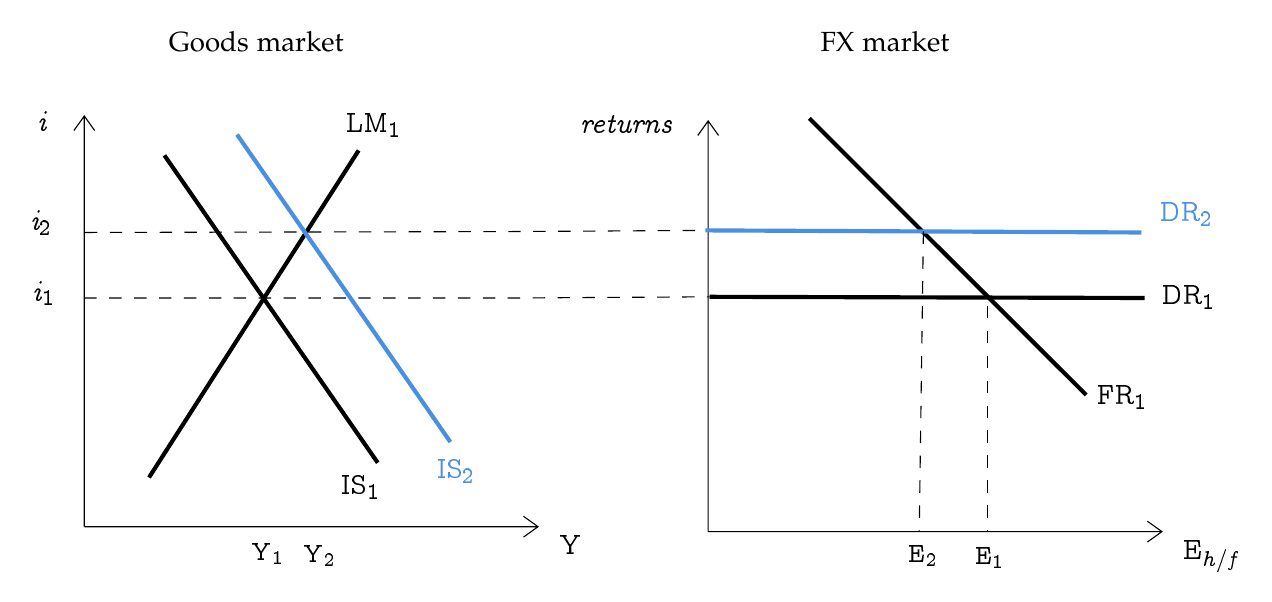
\begin{tikzpicture}[x=0.75pt,y=0.75pt,yscale=-1,xscale=1]
								%uncomment if require: \path (0,362); %set diagram left start at 0, and has height of 362
								
								%Shape: Axis 2D [id:dp7387221075140031] 
								\draw  (77.52,298.16) -- (296.13,298.16)(77.52,100.29) -- (77.52,298.16) -- cycle (289.13,293.16) -- (296.13,298.16) -- (289.13,303.16) (72.52,107.29) -- (77.52,100.29) -- (82.52,107.29)  ;
								%Straight Lines [id:da372006073802301] 
								\draw [color={rgb, 255:red, 0; green, 0; blue, 0 }  ,draw opacity=1 ][line width=1.5]    (116.13,119.25) -- (218.9,267.36) ;
								%Straight Lines [id:da1590002526416081] 
								\draw [line width=1.5]    (108.7,274.46) -- (209.7,116.88) ;
								%Shape: Axis 2D [id:dp7066322282955013] 
								\draw  (378.11,300.53) -- (596.73,300.53)(378.11,102.66) -- (378.11,300.53) -- cycle (589.73,295.53) -- (596.73,300.53) -- (589.73,305.53) (373.11,109.66) -- (378.11,102.66) -- (383.11,109.66)  ;
								%Straight Lines [id:da4775484258836953] 
								\draw [color={rgb, 255:red, 0; green, 0; blue, 0 }  ,draw opacity=1 ][line width=1.5]    (378.8,187.4) -- (588.42,187.97) ;
								%Straight Lines [id:da049078011774791985] 
								\draw  [dash pattern={on 4.5pt off 4.5pt}]  (77.52,187.97) -- (284.25,187.97) -- (378.8,187.4) ;
								%Straight Lines [id:da33935655662358744] 
								\draw [color={rgb, 255:red, 0; green, 0; blue, 0 }  ,draw opacity=1 ][line width=1.5]    (426.8,101.4) -- (560.19,234.66) ;
								%Straight Lines [id:da13296955473576566] 
								\draw [color={rgb, 255:red, 74; green, 144; blue, 226 }  ,draw opacity=1 ][line width=1.5]    (376.8,155.4) -- (586.8,156.41) ;
								%Straight Lines [id:da7855850150635582] 
								\draw  [dash pattern={on 4.5pt off 4.5pt}]  (77.8,156.4) -- (282.25,155.97) -- (376.8,155.4) ;
								%Straight Lines [id:da03982208723006364] 
								\draw  [dash pattern={on 4.5pt off 4.5pt}]  (481.8,155.9) -- (479.8,300.4) ;
								%Straight Lines [id:da7053160032413199] 
								\draw  [dash pattern={on 4.5pt off 4.5pt}]  (512.8,191.8) -- (512.8,300.41) ;
								%Straight Lines [id:da013387887657565933] 
								\draw [color={rgb, 255:red, 74; green, 144; blue, 226 }  ,draw opacity=1 ][line width=1.5]    (151.13,109.25) -- (253.9,257.36) ;
								
								% Text Node
								\draw (53.6,97.22) node [anchor=north west][inner sep=0.75pt]   [align=left] {$\displaystyle i$};
								% Text Node
								\draw (305.67,301.01) node [anchor=north west][inner sep=0.75pt]   [align=left] {$\displaystyle Y$};
								% Text Node
								\draw (202.42,97.94) node [anchor=north west][inner sep=0.75pt]   [align=left] {$\displaystyle LM_{1}$};
								% Text Node
								\draw (200.4,272.48) node [anchor=north west][inner sep=0.75pt]  [color={rgb, 255:red, 0; green, 0; blue, 0 }  ,opacity=1 ] [align=left] {$\displaystyle IS_{1}$};
								% Text Node
								\draw (315.39,98.77) node [anchor=north west][inner sep=0.75pt]   [align=left] {$\displaystyle returns$};
								% Text Node
								\draw (605.93,303.56) node [anchor=north west][inner sep=0.75pt]   [align=left] {$\displaystyle E_{h/f}$};
								% Text Node
								\draw (595.38,180.94) node [anchor=north west][inner sep=0.75pt]  [color={rgb, 255:red, 0; green, 0; blue, 0 }  ,opacity=1 ] [align=left] {$\displaystyle DR_{1}$};
								% Text Node
								\draw (51.51,178.97) node [anchor=north west][inner sep=0.75pt]   [align=left] {$\displaystyle i_{1}{}$};
								% Text Node
								\draw (117,58) node [anchor=north west][inner sep=0.75pt]   [align=left] {Goods market};
								% Text Node
								\draw (431,58) node [anchor=north west][inner sep=0.75pt]   [align=left] {FX market};
								% Text Node
								\draw (157.51,304.97) node [anchor=north west][inner sep=0.75pt]  [font=\small] [align=left] {$\displaystyle Y_{1}{}$};
								% Text Node
								\draw (473.51,305.97) node [anchor=north west][inner sep=0.75pt]  [font=\small] [align=left] {$\displaystyle E_{2}$};
								% Text Node
								\draw (563.84,228.93) node [anchor=north west][inner sep=0.75pt]  [color={rgb, 255:red, 0; green, 0; blue, 0 }  ,opacity=1 ] [align=left] {$\displaystyle FR_{1}$};
								% Text Node
								\draw (594.38,140.94) node [anchor=north west][inner sep=0.75pt]  [color={rgb, 255:red, 74; green, 144; blue, 226 }  ,opacity=1 ] [align=left] {$\displaystyle DR_{2}$};
								% Text Node
								\draw (50.51,144.97) node [anchor=north west][inner sep=0.75pt]   [align=left] {$\displaystyle i_{2}{}$};
								% Text Node
								\draw (505.51,307) node [anchor=north west][inner sep=0.75pt]  [font=\small] [align=left] {$\displaystyle E_{1}$};
								% Text Node
								\draw (246.4,264.48) node [anchor=north west][inner sep=0.75pt]  [color={rgb, 255:red, 74; green, 144; blue, 226 }  ,opacity=1 ] [align=left] {$\displaystyle IS_{2}$};
								% Text Node
								\draw (182.51,305.97) node [anchor=north west][inner sep=0.75pt]  [font=\small] [align=left] {$\displaystyle Y_{2}{}$};
									
							\end{tikzpicture}
										
					\end{framed}%
				}
				
				\fi
				
				\item Investors expect an appreciation of the home currency in the future.
				
				\ifAnswers
				
				{\color{Blue}
					\begin{framed}
						FR shifts left, IS shifts left, DR shifts down: Y $\downarrow$ , i $\downarrow$, E $\downarrow$, C $\downarrow$, I $\uparrow$, TB $\downarrow$ \\
						
							
							
							\tikzset{every picture/.style={line width=0.75pt}} %set default line width to 0.75pt        
							
							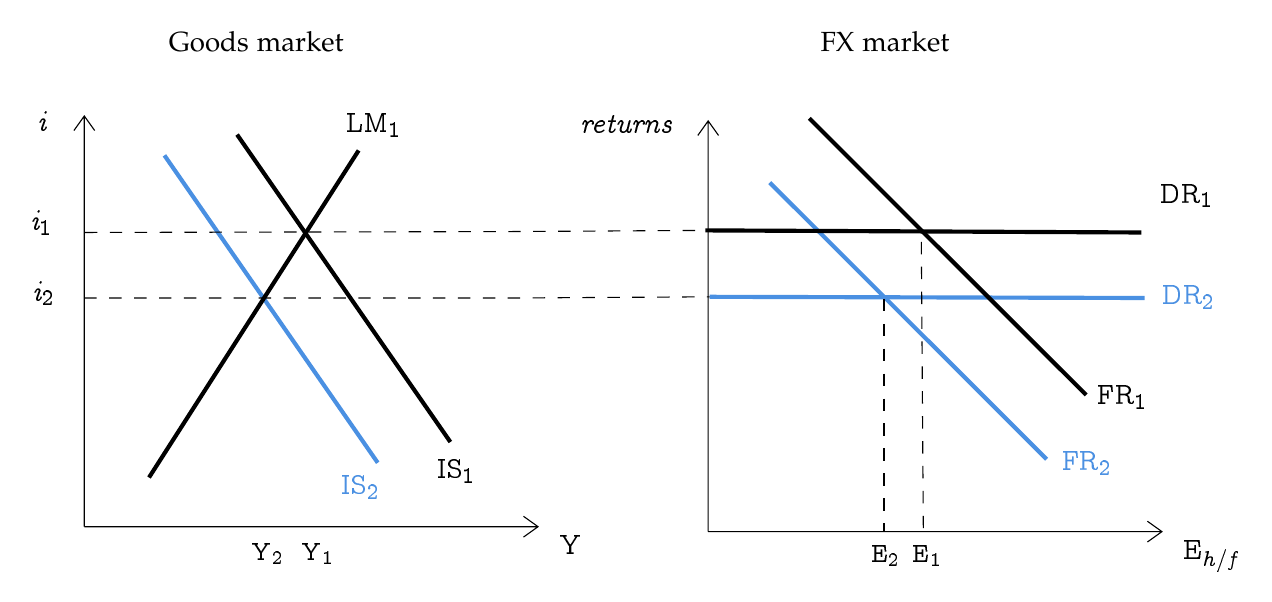
\begin{tikzpicture}[x=0.75pt,y=0.75pt,yscale=-1,xscale=1]
								%uncomment if require: \path (0,362); %set diagram left start at 0, and has height of 362
								
								%Shape: Axis 2D [id:dp7387221075140031] 
								\draw  (77.52,298.16) -- (296.13,298.16)(77.52,100.29) -- (77.52,298.16) -- cycle (289.13,293.16) -- (296.13,298.16) -- (289.13,303.16) (72.52,107.29) -- (77.52,100.29) -- (82.52,107.29)  ;
								%Straight Lines [id:da372006073802301] 
								\draw [color={rgb, 255:red, 74; green, 144; blue, 226 }  ,draw opacity=1 ][line width=1.5]    (116.13,119.25) -- (218.9,267.36) ;
								%Straight Lines [id:da1590002526416081] 
								\draw [line width=1.5]    (108.7,274.46) -- (209.7,116.88) ;
								%Shape: Axis 2D [id:dp7066322282955013] 
								\draw  (378.11,300.53) -- (596.73,300.53)(378.11,102.66) -- (378.11,300.53) -- cycle (589.73,295.53) -- (596.73,300.53) -- (589.73,305.53) (373.11,109.66) -- (378.11,102.66) -- (383.11,109.66)  ;
								%Straight Lines [id:da26983092411326215] 
								\draw [color={rgb, 255:red, 74; green, 144; blue, 226 }  ,draw opacity=1 ][line width=1.5]    (407.8,132.4) -- (541.19,265.66) ;
								%Straight Lines [id:da4775484258836953] 
								\draw [color={rgb, 255:red, 74; green, 144; blue, 226 }  ,draw opacity=1 ][line width=1.5]    (378.8,187.4) -- (588.42,187.97) ;
								%Straight Lines [id:da049078011774791985] 
								\draw  [dash pattern={on 4.5pt off 4.5pt}]  (77.52,187.97) -- (284.25,187.97) -- (378.8,187.4) ;
								%Straight Lines [id:da33935655662358744] 
								\draw [color={rgb, 255:red, 0; green, 0; blue, 0 }  ,draw opacity=1 ][line width=1.5]    (426.8,101.4) -- (560.19,234.66) ;
								%Straight Lines [id:da13296955473576566] 
								\draw [color={rgb, 255:red, 0; green, 0; blue, 0 }  ,draw opacity=1 ][line width=1.5]    (376.8,155.4) -- (586.8,156.41) ;
								%Straight Lines [id:da7855850150635582] 
								\draw  [dash pattern={on 4.5pt off 4.5pt}]  (77.8,156.4) -- (282.25,155.97) -- (376.8,155.4) ;
								%Straight Lines [id:da03982208723006364] 
								\draw  [dash pattern={on 4.5pt off 4.5pt}]  (462.8,188.41) -- (462.8,300.4) ;
								%Straight Lines [id:da7053160032413199] 
								\draw  [dash pattern={on 4.5pt off 4.5pt}]  (480.8,160.9) -- (481.8,304.41) ;
								%Straight Lines [id:da013387887657565933] 
								\draw [color={rgb, 255:red, 0; green, 0; blue, 0 }  ,draw opacity=1 ][line width=1.5]    (151.13,109.25) -- (253.9,257.36) ;
								
								% Text Node
								\draw (53.6,97.22) node [anchor=north west][inner sep=0.75pt]   [align=left] {$\displaystyle i$};
								% Text Node
								\draw (305.67,301.01) node [anchor=north west][inner sep=0.75pt]   [align=left] {$\displaystyle Y$};
								% Text Node
								\draw (202.42,97.94) node [anchor=north west][inner sep=0.75pt]   [align=left] {$\displaystyle LM_{1}$};
								% Text Node
								\draw (200.4,272.48) node [anchor=north west][inner sep=0.75pt]  [color={rgb, 255:red, 74; green, 144; blue, 226 }  ,opacity=1 ] [align=left] {$\displaystyle IS_{2}$};
								% Text Node
								\draw (315.39,98.77) node [anchor=north west][inner sep=0.75pt]   [align=left] {$\displaystyle returns$};
								% Text Node
								\draw (605.93,303.56) node [anchor=north west][inner sep=0.75pt]   [align=left] {$\displaystyle E_{h/f}$};
								% Text Node
								\draw (595.38,180.94) node [anchor=north west][inner sep=0.75pt]  [color={rgb, 255:red, 74; green, 144; blue, 226 }  ,opacity=1 ] [align=left] {$\displaystyle DR_{2}$};
								% Text Node
								\draw (546.84,260.93) node [anchor=north west][inner sep=0.75pt]  [color={rgb, 255:red, 74; green, 144; blue, 226 }  ,opacity=1 ] [align=left] {$\displaystyle FR_{2}$};
								% Text Node
								\draw (51.51,178.97) node [anchor=north west][inner sep=0.75pt]   [align=left] {$\displaystyle i_{2}{}$};
								% Text Node
								\draw (117,58) node [anchor=north west][inner sep=0.75pt]   [align=left] {Goods market};
								% Text Node
								\draw (431,58) node [anchor=north west][inner sep=0.75pt]   [align=left] {FX market};
								% Text Node
								\draw (157.51,304.97) node [anchor=north west][inner sep=0.75pt]  [font=\small] [align=left] {$\displaystyle Y_{2}{}$};
								% Text Node
								\draw (455.51,305.97) node [anchor=north west][inner sep=0.75pt]  [font=\small] [align=left] {$\displaystyle E_{2}$};
								% Text Node
								\draw (563.84,228.93) node [anchor=north west][inner sep=0.75pt]  [color={rgb, 255:red, 0; green, 0; blue, 0 }  ,opacity=1 ] [align=left] {$\displaystyle FR_{1}$};
								% Text Node
								\draw (594.38,131.94) node [anchor=north west][inner sep=0.75pt]  [color={rgb, 255:red, 0; green, 0; blue, 0 }  ,opacity=1 ] [align=left] {$\displaystyle DR_{1}$};
								% Text Node
								\draw (50.51,144.97) node [anchor=north west][inner sep=0.75pt]   [align=left] {$\displaystyle i_{1}{}$};
								% Text Node
								\draw (475.51,306) node [anchor=north west][inner sep=0.75pt]  [font=\small] [align=left] {$\displaystyle E_{1}$};
								% Text Node
								\draw (246.4,264.48) node [anchor=north west][inner sep=0.75pt]  [color={rgb, 255:red, 0; green, 0; blue, 0 }  ,opacity=1 ] [align=left] {$\displaystyle IS_{1}$};
								% Text Node
								\draw (181.51,304.97) node [anchor=north west][inner sep=0.75pt]  [font=\small] [align=left] {$\displaystyle Y_{1}{}$};
								
							\end{tikzpicture}
								
					\end{framed}%
				}
				
				\fi
				
			\end{enumerate}

\end{enumerate}

%\ifAnswers
%
%	\newpage
%
%	\begin{figure}[H] 
%		\centering
%		\caption{Plots for 4)}
%		\vspace*{-.2cm}
%		%\includegraphics[scale=0.735]{plots1.png} 
%	\end{figure}
%
%	\begin{figure}[H] 
%		\centering
%		\caption{Plots for 5}
%		\vspace*{-.2cm}
%		%\includegraphics[scale=0.735]{plots2.png} 
%	\end{figure}
%
%		\begin{figure}[H] 
%		\centering
%		\caption{Plots for 7}
%		\vspace*{-.2cm}
%		%\includegraphics[scale=0.735]{plots2.png} 
%	\end{figure}
%	
%
%\fi


\end{document} 